\begin{figure*}[htbp]
\centering
\subfigure[]
{
	\label{fig:berkeley_random_hum}
	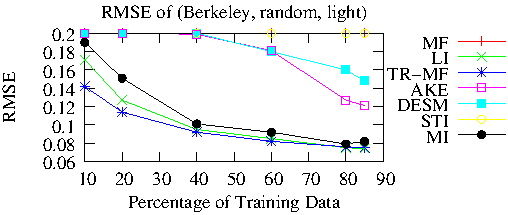
\includegraphics[scale=0.8]{table2_1_BRH}
}
\hspace{0in}
%\end{figure}
%\begin{figure}[H]
%\centering
\subfigure[]
{
	\label{fig:berkeley_random_light}
	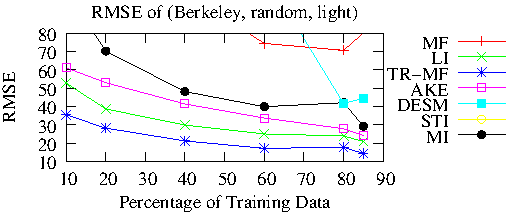
\includegraphics[scale=0.8]{table3_BRL}
}
\hspace{0in}
%\caption{}
%\end{figure}
%\begin{figure}[H]
%\centering
\subfigure[]
{
	\label{fig:berkeley_random_tem}
	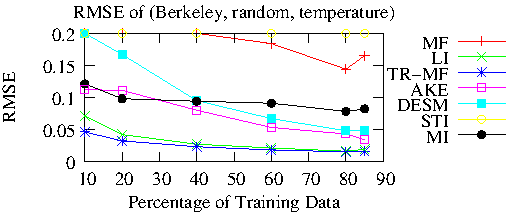
\includegraphics[scale=0.8]{table4_BRT}
}
\hspace{0in}
%\caption{}
%\end{figure}
%\begin{figure}[H]
%\centering
\subfigure[]
{
	\label{fig:traffic_random_hum}
	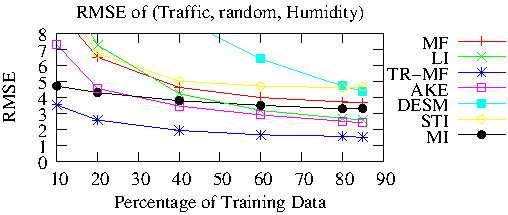
\includegraphics[scale=0.8]{table5_TRH}
}
\hspace{0in}
%\caption{}
%\end{figure}
%\begin{figure}[H]
%\centering
\subfigure[]
{
	\label{fig:traffic_random_tem}
	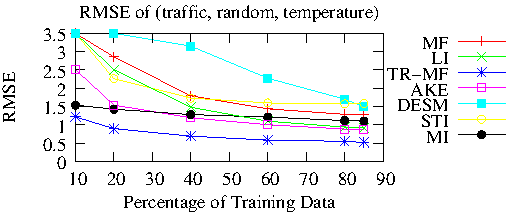
\includegraphics[scale=0.8]{table6_TRT}
}
\caption{Random Split}
\hspace{0in}
%\caption{}
\end{figure*}

%\begin{table*}
%%
%\begin{tabular}{cc}
%\subfigure[A]{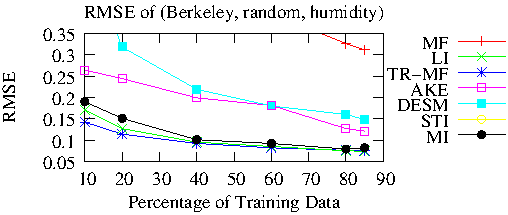
\includegraphics[scale=0.8]{table2_BRH}} 
%   & \subfigure[B]{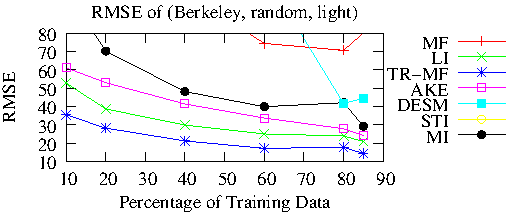
\includegraphics[scale=0.8]{table3_BRL}}\\
%\end{tabularx}
%\end{table*}
%\end{figure}
%\begin{figure}[H]
%\centering
%\mbox{
%\input{table11.pspdftex}}
%\caption{RMSE of (traffic, temporal, temperature}
%\end{figure}
\begin{figure*}[htbp]
\centering
\subfigure[]
{
	\label{fig:berkeley_temporal_hum}
	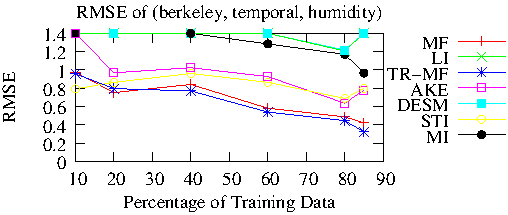
\includegraphics[scale=0.8]{table7_BTH}
}
\hspace{0in}
%\end{figure}
%\begin{figure}[H]
%\centering
\subfigure[]
{
	\label{fig:berkeley_temporal_light}
	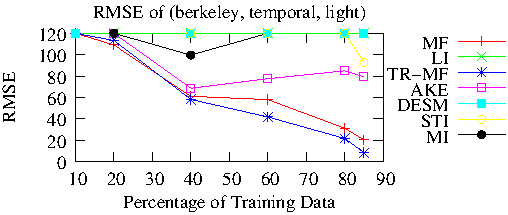
\includegraphics[scale=0.8]{table8_BTL}
}
\hspace{0in}
%\caption{}
%\end{figure}
%\begin{figure}[H]
%\centering
\subfigure[]
{
	\label{fig:berkeley_temporal_tem}
	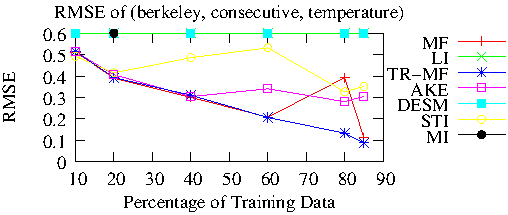
\includegraphics[scale=0.8]{table9_BTT}
}
\hspace{0in}
%%\caption{}
%%\end{figure}
%%\begin{figure}[H]
%%\centering
%\subfigure[]
%{
%	\label{fig:traffic_random_hum}
%	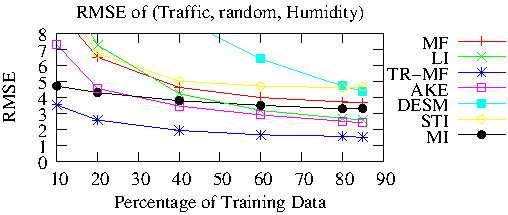
\includegraphics[scale=0.8]{table5_TRH}
%}
%\hspace{0in}
%%\caption{}
%%\end{figure}
%%\begin{figure}[H]
%%\centering
%\subfigure[]
%{
%	\label{fig:traffic_random_tem}
%	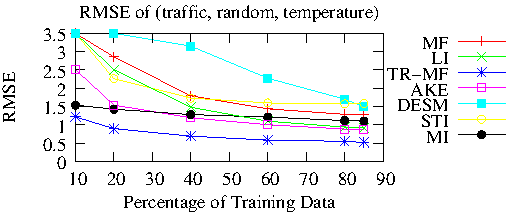
\includegraphics[scale=0.8]{table6_TRT}
%}
\caption{Temporal Split}
\hspace{0in}
%\caption{}
\end{figure*}